\documentclass[12pt,a4paper]{article}

\usepackage{fontspec}
\setmainfont{Latin Modern Roman}
\usepackage[english]{babel}
\usepackage[a4paper,margin=25mm]{geometry}
\usepackage{booktabs}
\usepackage{tabularx}
\usepackage{graphicx}
\usepackage{tikz}
\usetikzlibrary{arrows.meta}
\usepackage{hyperref}

% Настройка внешнего вида ссылок (чтобы убрать раздражающие цветные рамки)
\hypersetup{
	colorlinks=true,    % Включает цветной текст ссылок вместо рамок
	linkcolor=blue,     % Цвет внутренних ссылок (оглавление, формулы)
	urlcolor=cyan,      % Цвет внешних веб-ссылок
	citecolor=green     % Цвет ссылок на библиографию
}

\setlength{\parindent}{1.2em}
\setlength{\parskip}{0.3em}
\renewcommand{\arraystretch}{1.15}
\newcommand{\code}[1]{\textbf{\detokenize{#1}}}

\day=67
\title{Race master 4D: racist game\\[0.3em]
	\large Practical work documentation}
\author{Michael Gustavo \& Danila Malyshev}
\date{\today}

\begin{document}
	
	\maketitle
	
	\section{Clarified task}
	
	The project is a C++ program for simulating and displaying traffic at a
	four-way intersection. It models cars moving on several lanes in both
	directions, traffic lights for straight, left, and right movements, and
	pedestrians crossing the roads. The purpose is to observe queues and how they change when traffic and signal settings are changed.
	
	The program has two signal modes. In static mode, the green, yellow, and
	all-red pedestrian phase use selected durations. In automatic mode, green and
	pedestrian phase times depend on the waiting queues. The user can also change
	signal visibility, car speed limits, and the randomized car-arrival interval.
	Car speed limits and arrival intervals are sampled from uniform distributions
	within the selected ranges. In automatic mode, pedestrian arrivals also use a
	uniformly sampled interval, from 2.5 to 7 seconds.
	
	The current implementation builds four approaches, each with six lanes. Three
	lanes carry incoming traffic and three carry outgoing traffic. New cars are
	placed in a randomly selected available incoming lane, but each lane has a
	fixed movement, so cars do not choose a random turn. The model includes car
	following and signal stopping, but it does not yet include lane changes.
	Collisions are not simulated.
	
	For each new car, the speed limit is sampled uniformly from the selected speed
	range. Its initial speed is sampled from the selected minimum up to that
	vehicle's speed limit. Cars follow route waypoints, slow down behind other
	vehicles, stop for signals, and wait when a left turn conflicts with opposing
	traffic or the exit lane is blocked. A car is removed after completing its
	route.
	
	\section{Class diagram}
	
	The diagram shows the main active model classes and their relationships.
	Arrows marked with a number show how many objects are normally created.
	The dashed line is a signal reference, and the open triangle marks inheritance.
	
	\begin{figure}[htbp]
		\centering
		\resizebox{0.96\linewidth}{!}{%
			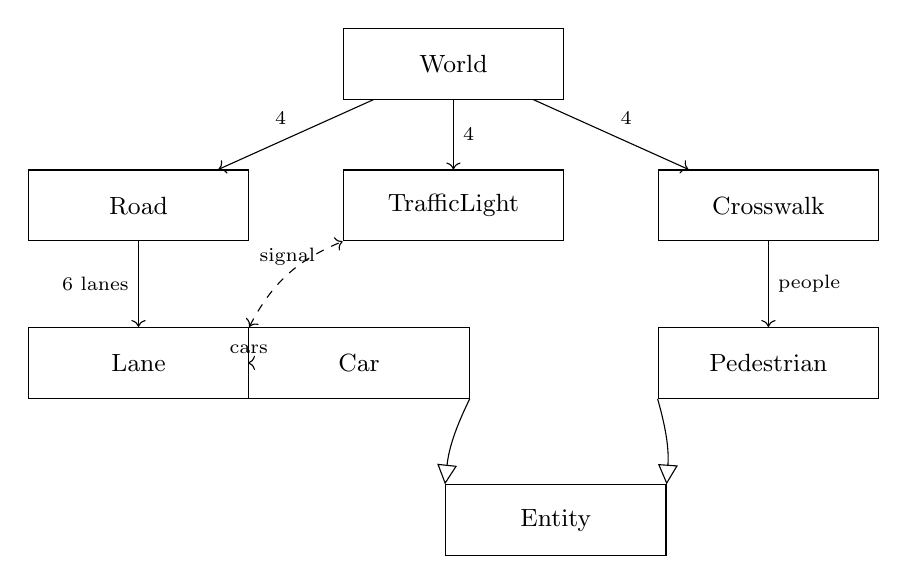
\begin{tikzpicture}[
				class/.style={
					draw,
					rectangle,
					align=center,
					minimum width=2.8cm,
					minimum height=9mm,
					font=\small
				},
				relation/.style={->},
				reference/.style={dashed,<->},
				inheritance/.style={-{Triangle[open,length=2.5mm,width=2.5mm]}} % <--- ИСПРАВЛЕНО ТУТ (добавлена ])
				]
				\node[class] (world) at (0,0) {World};
				\node[class] (road) at (-4,-1.8) {Road};
				\node[class] (light) at (0,-1.8) {TrafficLight};
				\node[class] (walk) at (4,-1.8) {Crosswalk};
				\node[class] (lane) at (-4,-3.8) {Lane};
				\node[class] (car) at (-1.2,-3.8) {Car};
				\node[class] (pedestrian) at (4,-3.8) {Pedestrian};
				\node[class] (entity) at (1.3,-5.8) {Entity};
				
				\draw[relation] (world) -- node[above left,font=\scriptsize]{4} (road);
				\draw[relation] (world) -- node[right,font=\scriptsize]{4} (light);
				\draw[relation] (world) -- node[above right,font=\scriptsize]{4} (walk);
				\draw[relation] (road) -- node[left,font=\scriptsize]{6 lanes} (lane);
				\draw[relation] (lane) -- node[above,font=\scriptsize]{cars} (car);
				\draw[relation] (walk) -- node[right,font=\scriptsize]{people} (pedestrian);
				\draw[reference] (lane.north east)
				to[bend left=20] node[above,font=\scriptsize]{signal} (light.south west);
				\draw[inheritance] (car.south east)
				to[bend right=10] (entity.north west);
				\draw[inheritance] (pedestrian.south west)
				to[bend left=10] (entity.north east);
			\end{tikzpicture} 
		}
		\caption{Main classes used by the simulation.}
	\end{figure}
	
	
	The \code{Crossroad} class exists in the source but is currently a placeholder,
	so it is not connected to the active model in the diagram.
	
	\section{Main class specifications}
	
	The following table gives a short description of the main classes and their
	public operations. The implementations are mostly in \code{objects.h}.
	
	\begin{center}
		\small
		\begin{tabularx}{\linewidth}{@{}p{2.2cm}X p{4.0cm}@{}}
			\toprule
			\textbf{Class} & \textbf{Purpose} & \textbf{Main operations} \\
			\midrule
			\code{Entity} &
			Common position, direction, velocity, speed, acceleration, and speed limit for
			moving objects. &
			\code{GetPos()}, \code{GetDirection()}, \code{GetSpeedLimit()}, and setters
			for speed and acceleration. \\
			\code{Car} &
			Inherits from \code{Entity}. Stores its lane, route, turn, current waypoint,
			and whether it is still active. Follows the route and reacts to signals and
			other cars. &
			\code{Car(Lane*)}, \code{Update(dt)}, \code{IsAlive()}, \code{Turn()},
			\code{StopAt()}. \\
			\code{Pedestrian} &
			Inherits from \code{Entity}. Stores a crossing path and moves along it at a
			fixed model speed of 5 km/h. &
			\code{SetPath(from,to)}, \code{Update(dt)}, \code{IsAlive()}. \\
			\code{Lane} &
			Stores road geometry, route waypoints, cars, a movement type, and references to
			a signal and exit lane. Also checks whether there is room for another car. &
			\code{Build(...)}, \code{HasRoom()}, \code{Update(dt)},
			\code{CurrentSignal()}. \\
			\code{Road} &
			Builds and owns the six lanes for one approach. &
			\code{Build(outward,n)}, \code{Update(dt)}, \code{GetLanes()}. \\
			\code{TrafficLight} &
			Stores the signal position, orientation, and current signal state, including
			protected left-turn states. &
			\code{GetSignal()}, \code{SetSignal()}, \code{GetPos()}. \\
			\code{Crosswalk} &
			Stores crossing endpoints and its pedestrians. It can create a pedestrian,
			check whether the crossing is busy, and update the people on it. &
			\code{Build(a,b)}, \code{Spawn()}, \code{Busy()}, \code{Update(dt)}. \\
			\code{World} &
			Builds and updates the four roads, lights, and crosswalks. It also controls
			signal phases, vehicle arrivals, and automatic pedestrian demand. &
			\code{Build()}, \code{Update(dt)}, \code{SetAutomaticSignals(bool)},
			\code{WaitingVehiclesForActivePhase()}. \\
			\code{Crossroad} &
			Placeholder for intersection geometry. It currently has no active behavior. &
			No active public interface. \\
			\code{background_manager} &
			Loads the available background textures and changes the image shown behind
			the simulation. &
			\code{Init_textures()}, \code{Get_background(...)},
			\code{Next_background(...)}. \\
			\bottomrule
		\end{tabularx}
	\end{center}
	
	\section{Tools and libraries}
	
	\begin{tabularx}{\linewidth}{@{}p{3.3cm}X@{}}
		\toprule
		\textbf{Item} & \textbf{Used in the project} \\
		\midrule
		Programming language & C++17. \\
		Graphics and window & SFML 3.0 (Graphics, Window, and System). \\
		User interface & ImGui-SFML. \\
		Build system & CMake 3.24 or later; the CMake project also checks for OpenGL. \\
		Development environment & Project source is in the Replit workspace. No separate
		C++ IDE is specified in the project files. \\
		Report editor & The report is set up for LuaLaTeX and can be opened in
		TeXstudio. \\
		\bottomrule
	\end{tabularx}
	
	\section{File structure}
	
	The source files are arranged as follows:
	
	\begin{verbatim}
		crossroads/
		|-- main.cpp
		|-- app.h
		|-- app.cpp
		|-- objects.h
		|-- objects.cpp
		|-- CMakeLists.txt
		`-- project_documentation.tex
	\end{verbatim}
	
	\code{main.cpp} starts the application by calling \code{app::run()}.
	\code{app.h} contains drawing declarations and the background manager.
	\code{app.cpp} creates the window, processes input, updates the world, and
	draws the simulation and ImGui controls. \code{objects.h} contains the model
	classes and most of their inline implementations. \code{objects.cpp} includes
	that header for the CMake target. \code{CMakeLists.txt} lists the program
	sources and external libraries.
	
	To build the program on a system with the required libraries installed, run:
	
	\begin{verbatim}
		cmake -S crossroads -B crossroads/build
		cmake --build crossroads/build
	\end{verbatim}
	
	\section{User interface}
	
	The program opens a 1200 by 800 pixel window. It displays the roads, cars,
	traffic lights, crosswalks, and pedestrians. The ImGui panel shows the active
	signal mode, the number of vehicles waiting for the current phase, and the
	pedestrian queue in automatic mode. A separate arrow section on the traffic
	light indicates a protected left-turn signal.
	
	The settings in the panel are listed below. Static signal durations only affect
	static mode. Changes to the speed range affect new cars.
	
	\begin{center}
		\begin{tabularx}{\linewidth}{@{}p{3.3cm}X@{}}
			\toprule
			\textbf{Control} & \textbf{Default and range} \\
			\midrule
			Signal mode & Static preset or automatic. \\
			Green duration & 12 s by default; slider range 1--90 s. \\
			Yellow duration & 3 s by default; slider range 1--15 s. \\
			Red / walk duration & 12 s by default; slider range 1--90 s. This is the
			all-red pedestrian phase. \\
			Signal visibility & 30 m by default; slider range 5--100 m. \\
			Car speed range & 30--120 km/h by default; values can be set from 5 to
			160 km/h. \\
			Car arrival interval & 4--8 s by default. Minimum slider: 1--30 s; maximum:
			from the selected minimum up to 60 s. \\
			\bottomrule
		\end{tabularx}
	\end{center}
	
	The world attempts to place one car on each road at startup. It then draws one
	random interval for the whole intersection and attempts to add one car to each
	road after that interval. Thus, all four roads use the same period. The program
	chooses an incoming lane with room; it skips an arrival if all lanes on that
	road are full. The \textbf{Add car} button attempts to add one car to every
	incoming lane with room. \textbf{Next background} changes the background image.
	The background manager expects image files under \code{../assets/}.
	
	\section{GitHub repository}
	
	The GituHub repository can be found \textbf{\href{https://github.com/WawandMG/Drunken-driver-simulator/tree/misha}{here}}. Main branch was hardly used (main is for losers), all the significant commits are located at the "Misha" branch.
\end{document}